\documentclass[15pt,a5paper,reqno]{article}
\usepackage{hyperref}
\usepackage[warn]{mathtext}
\usepackage[utf8]{inputenc}
\usepackage[T2A]{fontenc}
\usepackage[russian]{babel}
\usepackage{amssymb, amsmath, multicol}
\usepackage{graphicx}
\usepackage[shortcuts,cyremdash]{extdash}
\usepackage{wrapfig}
\usepackage{floatflt}
\usepackage{lipsum}
\usepackage{verbatim}
\usepackage{concmath}
\usepackage{euler}
\usepackage{xcolor}
\usepackage{etoolbox}
\usepackage{fancyhdr}
\usepackage{subfiles}
\usepackage{enumitem}
\usepackage{amsthm}
\usepackage{indentfirst}
\usepackage{import}

\DeclareMathOperator{\sign}{sign}

\RequirePackage[ left     = 1.5cm,
  right    = 1.5cm,
  top      = 2.0cm,
  bottom   = 1.25cm,
  includefoot,
  footskip = 1.25cm ]{geometry}
\setlength    {\parskip}        { .5em plus .15em minus .08em }
%\setlength    {\parindent}      { .0em }
\renewcommand {\baselinestretch}{ 1.07 }

\fancyhf{}

\renewcommand{\footrulewidth}{ .0em }
\fancyfoot[C]{\texttt{\textemdash~\thepage~\textemdash}}
\fancyhead[R]{\hfilШурыгин}

\makeatletter
\patchcmd\l@section{%
  \nobreak\hfil\nobreak
}{%
  \nobreak
  \leaders\hbox{%
    $\m@th \mkern \@dotsep mu\hbox{.}\mkern \@dotsep mu$%
  }%
  \hfill
  \nobreak
}{}{\errmessage{\noexpand\l@section could not be patched}}
\makeatother
\parindent = 1cm % отступ при красной строке⏎
\pagestyle{fancy}    
\renewcommand\qedsymbol{$\blacksquare$}

\newcommand{\when}[2]{
  \left. #1 \right|_{#2} \hspace
}
\renewcommand{\kappa}{\varkappa}
\RequirePackage{caption2}
\renewcommand\captionlabeldelim{}
\newcommand*{\hm}[1]{#1\nobreak\discretionary{}

\DeclareSymbolFont{T2Aletters}{T2A}{cmr}{m}{it}
{\hbox{$\mathsurround=0pt #1$}}{}}
% Цвета для гиперссылок
\definecolor{linkcolor}{HTML}{000000} % цвет ссылок
\definecolor{urlcolor}{HTML}{799B03} % цвет гиперссылок
 
\hypersetup{pdfstartview=FitH,  linkcolor=linkcolor,urlcolor=urlcolor, colorlinks=true}


%\setcounter{secnum[utf8x]depth}{0}

\begin{document}

% НАЧАЛО ТИТУЛЬНОГО ЛИСТА
\begin{center}
  {\small ФЕДЕРАЛЬНОЕ ГОСУДАРСТВЕННОЕ АВТОНОМНОЕ ОБРАЗОВАТЕЛЬНОЕ\\ УЧРЕЖДЕНИЕ ВЫСШЕГО ОБРАЗОВАНИЯ\\ МОСКОВСКИЙ ФИЗИКО-ТЕХНИЧЕСКИЙ ИНСТИТУТ\\ (НАЦИОНАЛЬНЫЙ ИССЛЕДОВАТЕЛЬСКИЙ УНИВЕРСИТЕТ)\\ ФИЗТЕХ-ШКОЛА РАДИОТЕХНИКИ И КИБЕРНЕТИКИ}\\
  \hfill \break
  \hfill \break
  \hfill \break
  \Huge{Изучение поглощения космических лучей в свинце}\\
\end{center}

\hfill \break
\hfill \break
\hfill \break
\hfill \break
\hfill \break
\hfill \break

\begin{flushright}
  \normalsize{Работу выполнил:}\\
  \normalsize{\textbf{Шурыгин Антон Алексеевич, группа Б01-909}}\\
\end{flushright}

\begin{center}
  \normalsize{\textbf{Долгопрудный, 2021}}
\end{center}


\thispagestyle{empty} % выключаем отображение номера для этой страницы

% КОНЕЦ ТИТУЛЬНОГО ЛИСТА

\newpage
\thispagestyle{plain}
\tableofcontents
\thispagestyle{plain}
\newpage


\paragraph{Цель работы:} измерить зависимость интенсивности космического излучения в лаборатории от толщины свинца.
\paragraph{Оборудование:} 


\section{Экспериментальная установка}

Основой установки является телескоп, отбирающий для регистрации лишь те частицы,
которые приходят в определенном направлении внутри телесного угла, определяемого
геометрией детекторов.
Установка состоит из двух детекторов частиц – сцинтилляционных счетчиков, набора
свинцовых фильтров и электронных схем, служащих для регистрации и дискриминации
сигналов от детекторов.


\begin{figure}[h]
    \centering
    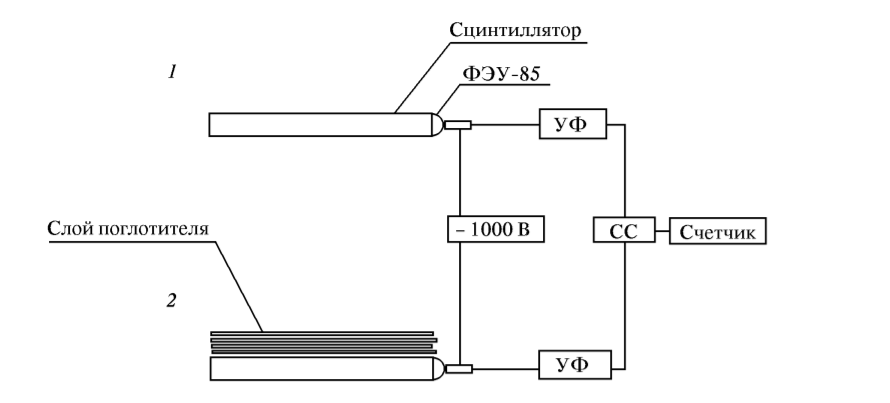
\includegraphics[width=1.0\linewidth]{pics/scheme.png}
    \caption{Схема экспериментальной установки}
    \label{scheme}
\end{figure}


Регистрация световых вспышек от сцинтилляторов производится с помощью ФЭУ-85,
напряжение питания на каждый ФЭУ подается от стабилизированного высоковольтного
выпрямителя. Сигналы с ФЭУ поступают на усилители-формирователи, а затем на схему
двойных совпадений. Схема совпадений формирует на выходе сигнал только в том
случае, если в обоих детекторах появились сигналы, совпадающие во времени в
интервале, равной разрешающему времени схемы. Число зарегистрированных импульсов
регистрируется пересчетным прибором.

\section{Ход работы и обработка данных}

Ниже представлены результаты измерений, число частиц измерялось за время 𝑡 = 900 с.


\begin{table}[h!]
    \centering
    \begin{tabular}{| c | c | c | c | c |}
\hline
$U, mV$ & $T_{room}, K$ & $T, K$ & $T_{br}, K$ & $ \sigma_{T}, K$\\
\hline
$39920$ & $298$ & $973,66$ & $1000$ & $ 28 $\\
\hline
\end{tabular}

    \caption{: данные для графика}
\label{tb1}
\end{table}

Известно, что мягкая (электронно-фотонная) компонента космического излучения почти
полностью поглощается слоем свинца толщиной 10 − 15 см, а жесткая (мюонная) –
практически не поглощается. Имея это в виду, вычитаем из значений $n$ на предыдущем
графике значение, соответствующее $d$ = 131 мм.

\begin{table}[h!]
    \centering
    \begin{tabular}{| c | c | c | c | c |}
\hline
$U, mV$ & $T_{room}, K$ & $T, K$ & $T_{br}, K$ & $ \sigma_{T}, K$\\
\hline
$39920$ & $298$ & $973,66$ & $1000$ & $ 28 $\\
\hline
\end{tabular}

    \caption{: данные для графика}
    \label{tb2}
\end{table}

Построим графики зависимости по таблицам 1, 2}.

\begin{figure}[h!]
    \centering
    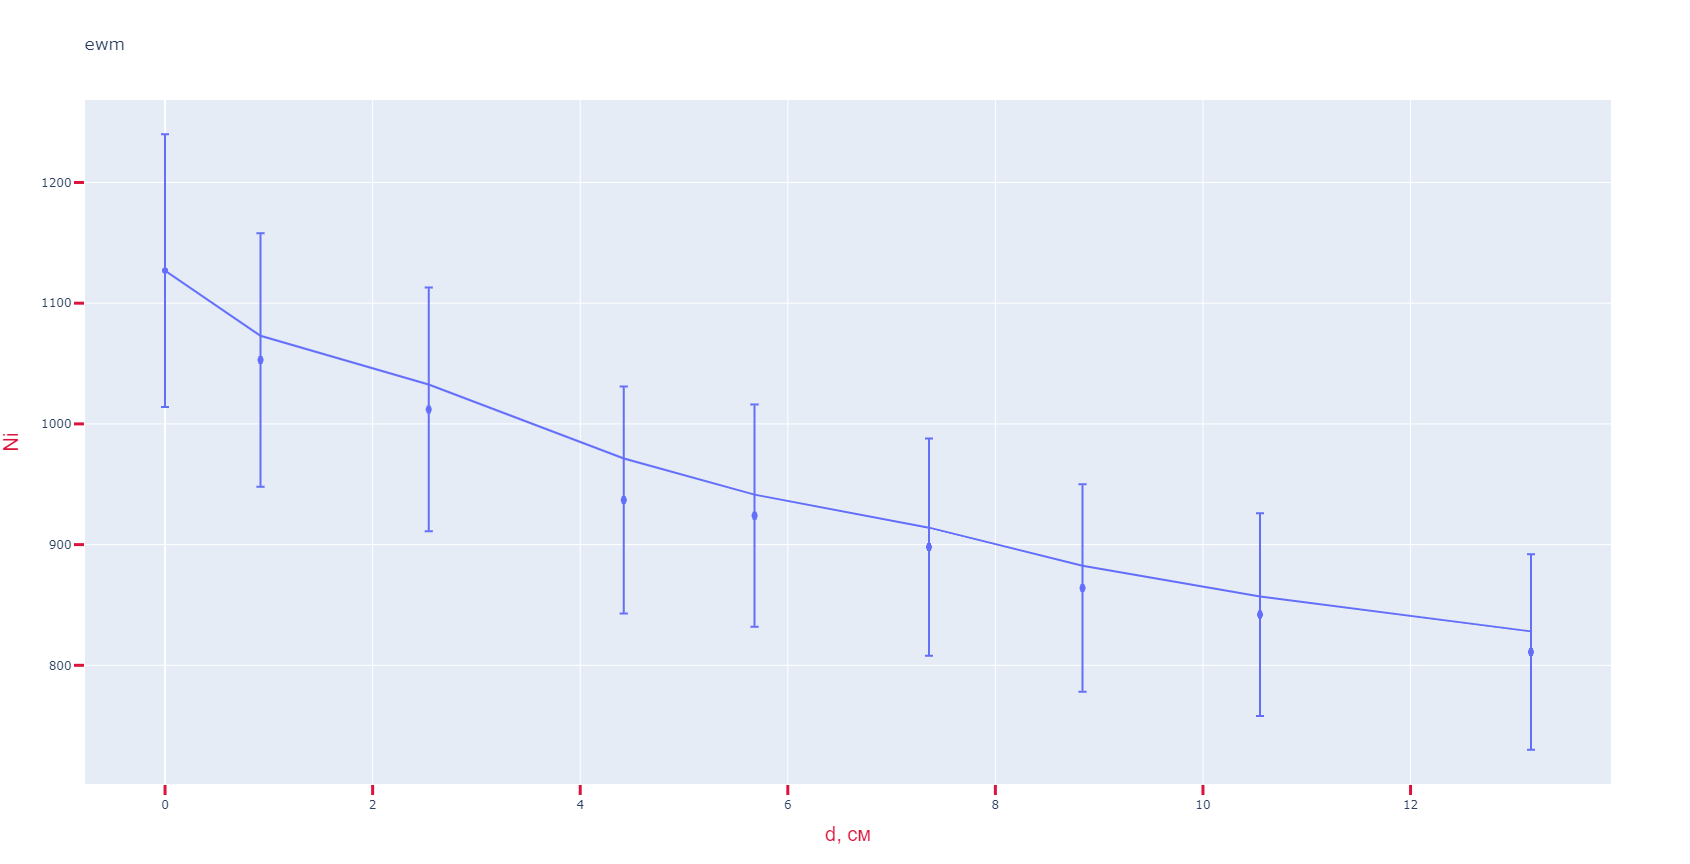
\includegraphics[width=1.0\linewidth]{pics/lab_5_7_4(1).png}
    \caption{Зависимость числа прошедших частиц от толщины свинца}
    \label{graph}
\end{figure}

\begin{figure}[h!]
    \centering
    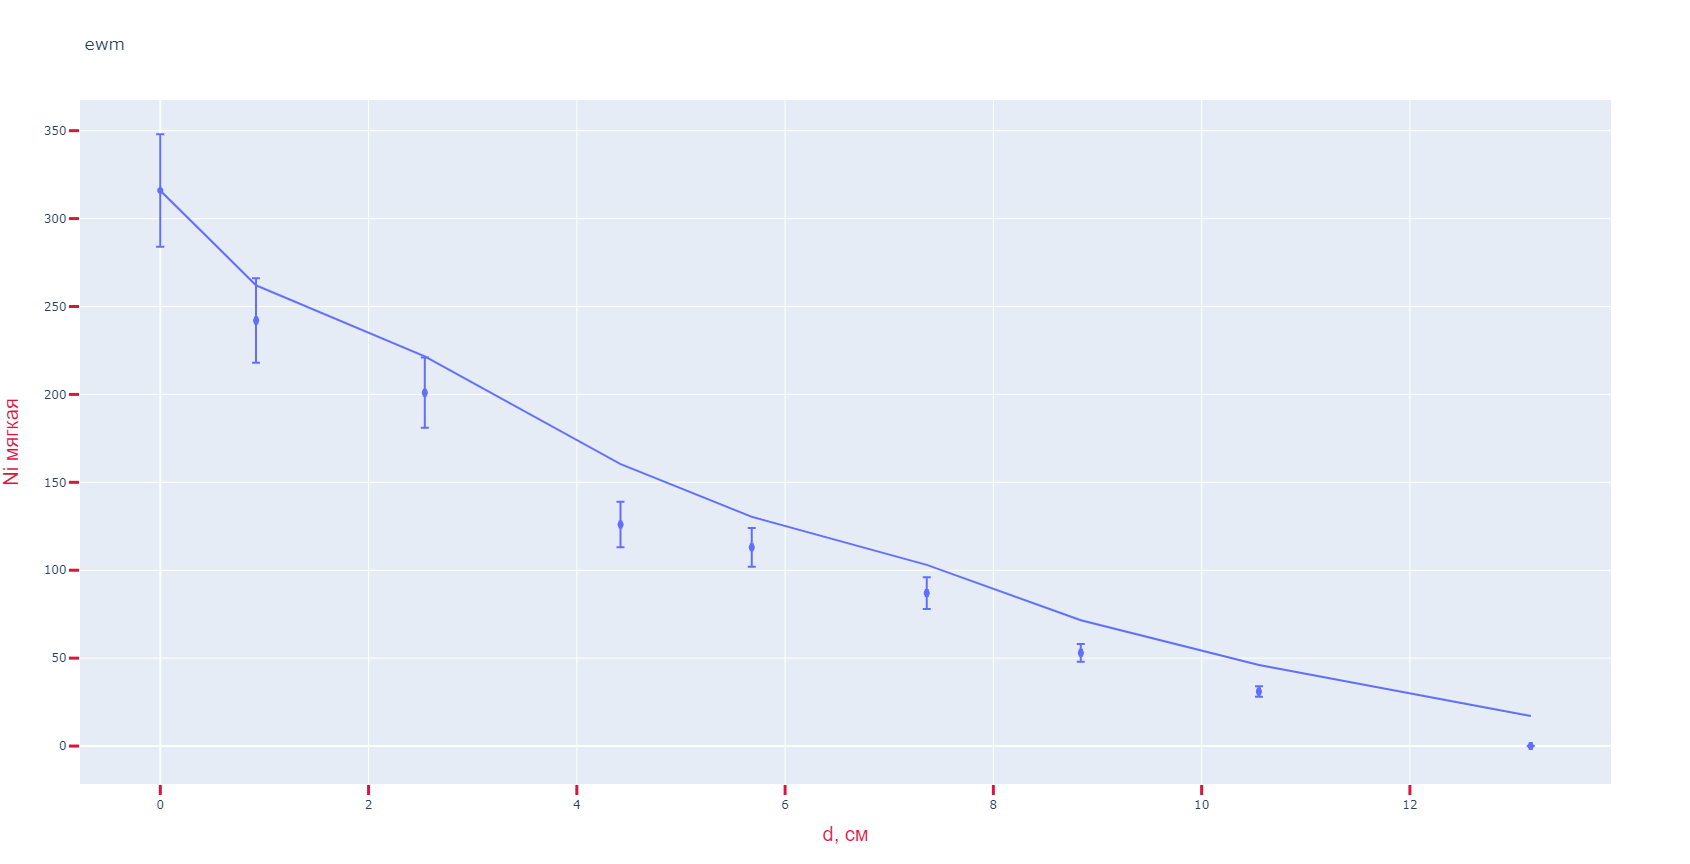
\includegraphics[width=1.0\linewidth]{pics/lab_5_7_4(2).png}
    \caption{Зависимость числа прошедших частиц (мягкая компонента) от толщины свинца}
    \label{graph}
\end{figure}

\end{document}